\documentclass[12pt]{article}
\usepackage[margin=1.0in]{geometry}
\usepackage{graphicx}
\usepackage{subcaption}
\usepackage{cleveref}
\usepackage{indentfirst}
\usepackage{amsmath}
\usepackage{listings}
\usepackage[title]{appendix}
\usepackage{siunitx} % Required for alignment
\usepackage{mdframed}

\begin{document}

	
\begin{center}
	\huge{Exploring the Effects of the Adaptive Cosine Estimator on Convolutional Neural Network Performance for Hyperspectral Imagery Classification} \\
	\vspace{5mm}
	\large{Alex Hurt}
\end{center}

%1) ABSTRACT. why care, what method did you use, what data did you explore, what did you find!
%
\section{Abstract}

Hyperspectral Imagery (HSI) Classification is a difficult but important task in Remote Sensing.
%
As hyperspectral sensors become more popular, the ability to perform classification at the hyperspectral level will grow more and more important.
%
HSI has many challenges that other image sources (i.e. RGB) do not have, such as labeling at the pixel level rather than image level and a so-called curse of dimensionality.
%
In recent years, several researchers have attempted to perform HSI classification with a variety of methods.
%
With the rise of deep learning, one of the most popular methods for HSI classification is Convolutional Neural Networks (CNN).
%
While HSI have several inherent challenges, so too do Convolutional Neural Networks, and understanding the limitations of CNN is critical to building a well performing classifier.
%
Recently, researchers have tried several tweaks to the standard CNN to improve HSI classification performance, such as using deformable convolutions by Zhu \textit{et al.} \cite{zhu_deformable_2018}. 
%
Another approach was taken by Paoletti \textit{et al.}, who used a CNN combined with capsule networks for HSI classification \cite{paoletti_capsule_2018}.

While numerous approaches have been taken for HSI classification, most techniques do not utilize the amount of spectral information contained in HSI when performing classification.
%
To that end, I will utilize a method of detection in HSI given sample object signatures, known as the Adaptive Cosine Estimator (ACE).
%
ACE allows detection and produces scoring at the pixel level within HSI given the signature of the objects of interest. 
%
In this project, I will combine the ACE technique with a CNN to produce a custom neural network architecture that involves preprocessing samples with ACE, named \textit{ACENet}.
%
ACENet combines the spectral classification methods of ACE with the spatial classification methods utilized by CNN to produce an architecture that can better classify HSI.
%
More details of this new architecture are described in Section \ref{sec:methods}.
%
Following the description of methods, I describe the data used for experimentation in Section \ref{sec:data} and then the design, results, and analysis of experiments in \ref{sec:experiments} before drawing final conclusions in Section \ref{sec:conclusion}.


%2) METHODS. describe your algorithm(s). your goal, show me you KNOW it
%
\section{Methods}\label{sec:methods}
To explore the effects of ACE on CNN Performance, I first move to introduce the data preprocessing that is performed prior to input to the CNN.
%
Since most hyperspectral datasets are labeled at the pixel label, the first step of preprocessing is to extract patches from the dataset.
%
To do this, parameters of window size and stride are selected and then used to extract patches of size window size by window size, and then sliding a number of pixels defined by stride.
%
Each patch is then normalized between 0 and 1 and fed into ACENet.

The ACENet architecture has two different modes: with or without ACE.
%
The only difference between the two is in the non-ACE mode, each patch is fed in raw and the input size to the first convolutional layer is (w x w x b) where w is the window size and b is the number of bands in the hyperspectral dataset.
%
Meanwhile, the ACE mode has another step between preprocessing and the first convoutional layer known as the ACELayer.
%
The ACELayer uses the dataset and ground truth to calculate a mean signal for each class in the dataset.
%
ACE is then run on each patch with each class's mean signal as the target signal. 
%
The resulting matrices are concatenated to form a single input sample with shape (w x w x n) where w is the window size and n is the number of classes, which is also the input shape of the first convolutional layer.
%
Both modes of ACENet have the same number of samples, but the ACE enabled mode has a reduction of dimensionality due to the number of classes being less than number of bands in HSI, but also has added computation of transforming samples from HSI pixels to the concatenation of ACE results.

Both ACE enabled and ACE disabled modes of ACENet have identical architectures beginning at the first convolutional layer.
%
The framework developed for this architecture is parameterized to allow for an arbitrary number of convolutional layers so that an optimal setting may be found for a given dataset.
%
Following the final convolutional layer, there is a single Max Pooling layer that feeds into a flattening layer.
%
Now that all feature extraction is finished, the flattened features are fed into the first fully connected layer composed of 256 units.
%
Next, a 25\% dropout layer is added in an attempt to add generalizability and improve cross validation performance.
%
Another fully connected layer follows the dropout layer before the final softmax layer for classification.



%3) DATA. document your data
%
\section{Data}\label{sec:data}
For this project, I chose to use the ever popular HSI benchmark dataset Indian Pines (IP) \cite{IP}.
%
IP is a HSI dataset composed of 220 hyperspectral bands that was collected in 1992 and has been used in a variety of research.
%
The dataset has shape of 144x144, and is one of few HSI datasets that has excellent pixel level ground truth data.
%
Use of this dataset will allow for easy comparison of this method with other methods due to the high popularity of IP.
%
The IP dataset is distributed as MatLab files and has 16 agricultural classes within it.

%4) EXPERIMENTS and RESULTS. what did you run and what did you find. Yes, document, but I want to see your ANALYSIS!
%
\section{Experiments}\label{sec:experiments}

In an effort to test the usability of ACENet, several experiments were run with several different parameters, both in ACE enabled and ACE disabled modes. 
%
The first set of experiments were done to test how stride and window size affected validation testing of CNN on HSI in general, and then another was run to explore how those same two parameters affected results with ACE enabled.
%
After finding ideal sets of window and stride sizes and exploring how ACE enabled CNN perform against Non-ACE enabled CNN, I investigate what the optimal number of convolutional layers is for feature extraction in HSI imagery.
%
All experiments are run using the IP dataset and are run using a Keras/TensorFlow software stack on a server with 4 NVIDIA Tesla V100s and 80 logical processors.
%
Network parameters were held constant with an initial learning rate of 0.01 and decay of 1e-6 along with a momentum of 0.9 in a Stochastic Gradient Descent (SGD) optimizer and categorical cross entropy loss function.
% 

\subsection{Varied Window and Stride Sizes}
Due to the pixel level labeling seen in the IP dataset and the necessity of CNN to have some NxN patch of input, it is a useful task to vary the input patch size and observe how that change impacts CNN performance. 
%
A balance must be struck between computational complexity and context around a pixel.
%
If the window size is too small, then there is not enough context, and performance is hindered, while a window size too large will result in more complex calculations with higher training times and may lead to a performance hit as well depending if the chosen size contains too much context relative to the labeled pixel.
%
To that end, I adjust the window size $w$ from 5x5 up to 11x11 in 2x2 increments, and set the stride for each experiment to $\lfloor\frac{w}{2}\rfloor$. 
%
I set ACENet to run in ACE disabled mode, and use 15 convolutional layers and train for 100 epochs on 80\% of the data.
%
I use the remaining 20\% of as validation data.
%
The results of this experiment are shown in Figure \ref{figure:noace}.

\begin{figure*}
	\label{figure:noace}
	\centering
	\caption{ACENet results on IP after 80/20 validation split using various window and stride sizes}
	\begin{subfigure}{0.45\linewidth}
		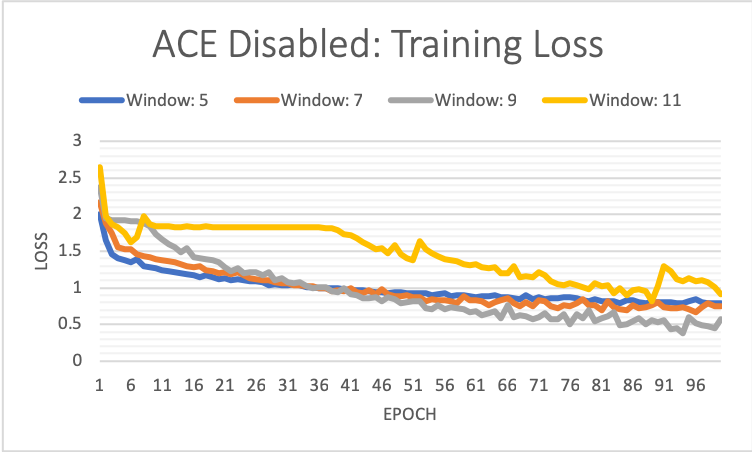
\includegraphics[width=\linewidth]{ace-disabled-loss.png}
		\caption{Training Loss}
	\end{subfigure}
	\hfill
	\begin{subfigure}{0.45\linewidth}
		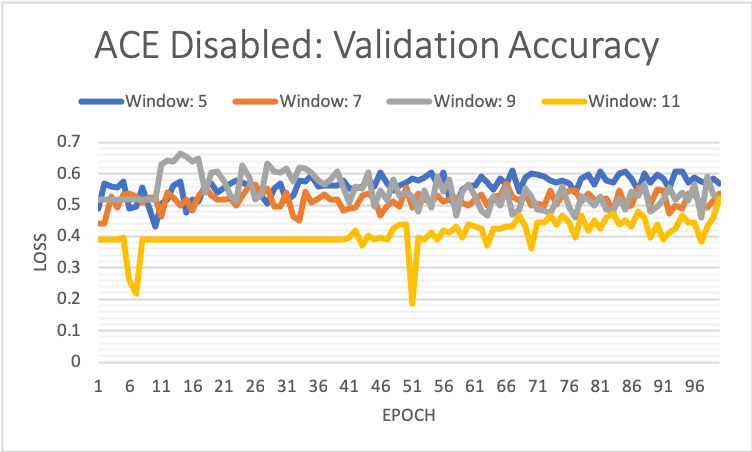
\includegraphics[width=\linewidth]{ace-disabled-valacc.png}
		\caption{Training Loss}		
	\end{subfigure}
\end{figure*}



\begin{figure*}
	\label{figure:withace}
	\centering
	\caption{ACENet results on IP after 80/20 validation split using various window and stride sizes}
	\begin{subfigure}{0.45\linewidth}
		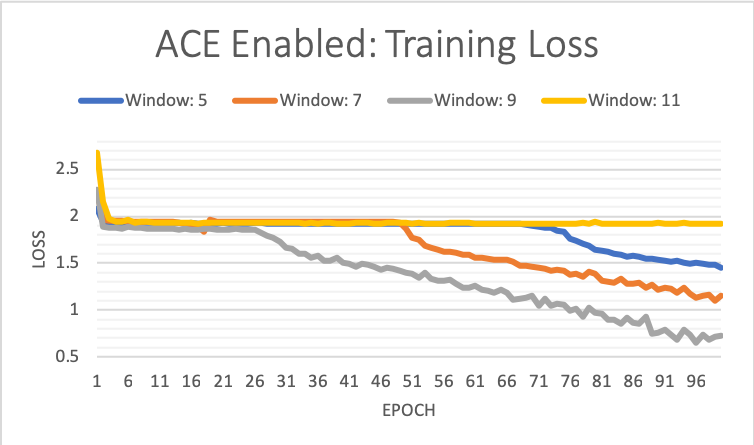
\includegraphics[width=\linewidth]{ace-enabled-loss.png}
		\caption{Training Loss}
	\end{subfigure}
	\hfill
	\begin{subfigure}{0.45\linewidth}
		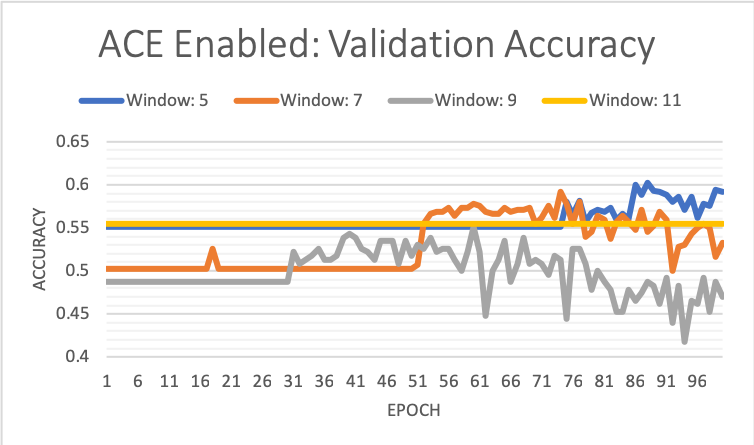
\includegraphics[width=\linewidth]{ace-enabled-valacc.png}
		\caption{Training Loss}		
	\end{subfigure}
\end{figure*}

As Figure \ref{figure:noace} shows, the results of ACE Disabled HSI classification are not extraordinary.
%
The best validation accuracy is a measly 0.664, which occurs with a window size of 9 after 14 epochs of training.
%

\subsection{ACE Enabled vs. ACE Disabled}
\subsection{Ideal Network Size}

%5) CONCLUSIONS. summarize it folks!
\section{Conclusion}\label{sec:conclusion}


%%%%%%%%%%%%%%%%
%		 REFERENCES
%%%%%%%%%%%%%%%%%
\newpage
\bibliography{refs} 
\bibliographystyle{ieeetr}


\end{document}
